% ****** Start of file apssamp.tex ******
%
%   This file is part of the APS files in the REVTeX 4.1 distribution.
%   Version 4.1r of REVTeX, August 2010
%
%   Copyright (c) 2009, 2010 The American Physical Society.
%
%   See the REVTeX 4 README file for restrictions and more information.
%
% TeX'ing this file requires that you have AMS-LaTeX 2.0 installed
% as well as the rest of the prerequisites for REVTeX 4.1
%
% See the REVTeX 4 README file
% It also requires running BibTeX. The commands are as follows:
%
%  1)  latex apssamp.tex
%  2)  bibtex apssamp
%  3)  latex apssamp.tex
%  4)  latex apssamp.tex
%
\documentclass[%
 reprint,
%superscriptaddress,
%groupedaddress,
%unsortedaddress,
%runinaddress,
%frontmatterverbose, 
%preprint,
%showpacs,preprintnumbers,
%nofootinbib,
%nobibnotes,
%bibnotes,
 amsmath,amssymb,
 aps,
%pra,
%prb,
%rmp,
%prstab,
%prstper,
%floatfix,
10.5pt,
]{revtex4-1}

\usepackage{graphicx}% Include figure files
\usepackage{subfigure}
\usepackage{multirow}
\usepackage{array}
\usepackage{dcolumn}% Align table columns on decimal point
\usepackage{bm}% bold math
%\usepackage{hyperref}% add hypertext capabilities
%\usepackage[mathlines]{lineno}% Enable numbering of text and display math
%\linenumbers\relax % Commence numbering lines

%\usepackage[showframe,%Uncomment any one of the following lines to test 
%%scale=0.7, marginratio={1:1, 2:3}, ignoreall,% default settings
%%text={7in,10in},centering,
%%margin=1.5in,
%%total={6.5in,8.75in}, top=1.2in, left=0.9in, includefoot,
%%height=10in,a5paper,hmargin={3cm,0.8in},
%]{geometry}

\usepackage{xeCJK}
\setCJKmainfont[ItalicFont={KaiTi}, BoldFont={KaiTi}]{KaiTi}
\usepackage{textcomp}
\usepackage{chemfig}
\usepackage[version=4]{mhchem}
\usepackage{fontspec}
\usepackage{listings}
\usepackage{xcolor}
\usepackage{xcolor} % 定制颜色
\definecolor{mygreen}{rgb}{0,0.6,0}
\definecolor{mygray}{rgb}{0.5,0.5,0.5}
\definecolor{mymauve}{rgb}{0.58,0,0.82}
\lstset{
backgroundcolor=\color{white},      % choose the background color
basicstyle=\footnotesize\ttfamily,  % size of fonts used for the code
columns=fullflexible,
tabsize=4,
breaklines=true,               % automatic line breaking only at whitespace
captionpos=b,                  % sets the caption-position to bottom
commentstyle=\color{mygreen},  % comment style
escapeinside={\%*}{*)},        % if you want to add LaTeX within your code
keywordstyle=\color{blue},     % keyword style
stringstyle=\color{mymauve}\ttfamily,  % string literal style
frame=single,
rulesepcolor=\color{red!20!green!20!blue!20},
% identifierstyle=\color{red},
language=Mathematica,
}

\usepackage[normalem]{ulem}

\newcommand{\chuhao}{\fontsize{42pt}{44.9pt}\selectfont}    % 初号, 1.5倍行距
\newcommand{\xiaochu}{\fontsize{30pt}{40pt}\selectfont}    % 小初, 1.5倍行距
\newcommand{\yihao}{\fontsize{26pt}{36pt}\selectfont}    % 一号, 1.4倍行距
\newcommand{\erhao}{\fontsize{22pt}{28pt}\selectfont}    % 二号, 1.25倍行距
\newcommand{\xiaoer}{\fontsize{18pt}{18pt}\selectfont}    % 小二, 单倍行距
\newcommand{\sanhao}{\fontsize{16pt}{24pt}\selectfont}    % 三号, 1.5倍行距
\newcommand{\xiaosan}{\fontsize{15pt}{22pt}\selectfont}    % 小三, 1.5倍行距
\newcommand{\sihao}{\fontsize{14pt}{21pt}\selectfont}    % 四号, 1.5倍行距
\newcommand{\sihaox}{\fontsize{14pt}{28pt}\selectfont}    % 四号, 1.5倍行距
\newcommand{\banxiaosi}{\fontsize{13pt}{19.5pt}\selectfont}    % 半小四, 1.5倍行距
\newcommand{\xiaosix}{\fontsize{12pt}{24pt}\selectfont} 	% 小四, 1.5倍行距
\newcommand{\xiaosi}{\fontsize{12pt}{18pt}\selectfont}     
\newcommand{\dawuhao}{\fontsize{11pt}{11pt}\selectfont}    % 大五号, 单倍行距
\newcommand{\wuhao}{\fontsize{10.5pt}{10.5pt}\selectfont}    % 五号, 单倍行距
\newcommand{\xiaowu}{\fontsize{9pt}{9pt}\selectfont}    % 五号, 单倍行距

%\usepackage[fntef]{ctexcap}
%\CTEXsetup[number={\chinese{section}、},format={\Large\bfseries}]{section}
\setCJKfamilyfont{fangsong}{FangSong}                      %仿宋2312 fs  
\newcommand{\fangsong}{\CJKfamily{fangsong}}  

\usepackage{wrapfig}
\usepackage{fancyhdr}
\usepackage{fancybox}   






\newcommand{\bra}[1]{\langle #1 |}
\newcommand{\ket}[1]{| #1 \rangle}
\newcommand{\bracket}[2]{\langle #1 | #2 \rangle}
\newcommand{\bracketl}[3]{\langle #1 | #2 | #3 \rangle}
\newcommand{\func}{\mathrm \,}
\newcommand{\define}[2]{
	\begin{definition}
	\begin{description}
	\item[#1]
	#2
	\end{description}
	\end{definition}
}

\newcommand{\sch}{Schr\"odinger}
\newcommand{\grad}{\nabla}
\newcommand{\ueq}{\neq}
\newcommand{\celsius}{\ensuremath{^\circ\hspace{-0.09em}\mathrm{C}}}
\newcommand{\unit}[2]{#1 \, \mathrm{#2}}

\begin{document}

%\preprint{APS/123-QED}

\title{The concealed truth behind equilibrium}% Force line breaks with \\
%\thanks{A footnote to the article title}% give thanks

\author{Rui Li}
 %\altaffiliation[Also at ]{Physics Department, XYZ University.}%Lines break automatically or can be forced with \\
%\author{Second Author}%
%\email{3160102098@zju.edu.cn}
\affiliation{%
 Qiushi science class (chemistry)\\
 Chu Kochen Honor College
}%

%\collaboration{MUSO Collaboration}%\noaffiliation

%\author{Zong Wei Huang}
% \homepage{http://www.Second.institution.edu/~Charlie.Author}
%\affiliation{
% Second institution and/or address\\
% This line break forced% with \\
%}%
%\affiliation{
%Qiushi science class (chemistry)\\
% Chu Kochen Honor College
%}%
%\author{Delta Author}
%\affiliation{%
% Authors' institution and/or address\\
% This line break forced with \textbackslash\textbackslash
%}%

%\collaboration{CLEO Collaboration}%\noaffiliation

%\date{\today}% It is always \today, today,
             %  but any date may be explicitly specified

\begin{abstract}
Relation between equilibrium and temperature is investigated. The assumption of ideal-gas behavior and invariability of $\Delta_rH_m$ is verified and help achieve great linearity of $\ln{p}$ or $\ln{K^\ominus}$ towards $1/T$. Machine learning method is utilized to apply Antoine method, which fails to give satisfying results.
\end{abstract}

%\pacs{Valid PACS appear here}% PACS, the Physics and Astronomy
                             % Classification Scheme.
\keywords{Clausius methods, Antoine methods, Equilibrium}%Use showkeys class option if keyword
                              %display desired
\maketitle

\tableofcontents

\section{Introduction}
Ammonium carbamate, being an intermidiate for the synthesis of urea, is remarkable due to its ability to decompose,
\begin{center}
\ce{NH2COONH4(s) <=> 2 NH3(g) + CO2(g)}
\end{center}
It is a perfect approximation that the chemical potential of a solid substance is constant, which leads to the obvious conclusion that the reaction is dominated by the chemical potential of the gases produced. Regarding them as ideal gases, we get the chemical potential of them,
\begin{equation}
\mu_B =\left(\frac{\partial G}{\partial n_B} \right)_{p,T,n_C} = RT\ln{p_B}
\end{equation}
w.r.t. the Gibbs free energy of an ideal gas,
\begin{equation}
d G_\text{ideal} = Vdp\,\Big|_{dT=0} = \frac{nRT}{p} dp \Big|_{dT=0} = nRT \, d\ln{p}\,\Big|_{dT=0}
\end{equation}
and the assumpution that there is no interaction among ideal gases.

When a reaction reaches its equilibrium, it follows
\begin{equation}
dG =0 \Rightarrow \Delta_r G_m d n + \sum_B \mu_B d n = 0
\end{equation}
and that
\begin{equation}
d n_r = - k_r d n , \quad d n_p = k_p d n
\end{equation}
where $r$ stands for reactants and $p$ for products, and $k$ refers to the coefficient of the matter assigned in the chemical reaction.
Thus $K$ is defined as
\begin{equation}
K = \prod_B  p_B^{k_B}
\end{equation}
and
\begin{equation}
K^\ominus = \left(\frac{p_B}{p^\ominus}\right)^{k_B}
\end{equation}
with reference to the standard state. Thus
\begin{equation}
\Delta_r G_m^\ominus = -RT \ln{K^\ominus}
\end{equation}

\begin{equation}
-RT \ln{K} = \Delta_r G_m = \Delta_r H_m - T \Delta_r S_m
\end{equation}
\begin{equation}
\ln{K} =- \frac{\Delta_r H_m^\ominus}{RT} + \frac{\Delta S_m}{R}
\end{equation}
It is assumed that $\Delta_\text{r} H_m$ as well as $\Delta_\text{r} S_m$ does not vary with temperature, then
\begin{equation}
\frac{d \ln{K}}{dT} = \frac{\Delta_r H_m ^\ominus}{RT^2}
\end{equation}
After integration, we obtain
\begin{equation}
\ln{K} = -\frac{\Delta_r H_m^\ominus}{RT} + \mathrm{constant}
\end{equation}

Vaporization is another kind of equilibrium, namely the equilibrium between liquid phase and gas phase.  During vaporization the temperature remains constant, and it is assumed that $\Delta_\text{vap} H_m^\ominus$ is constant, thus
\begin{equation}
RT d \ln{p_B} =d \mu_B = S_m dT  = \frac{\Delta_\text{vap} H_m}{T} dT
\end{equation}
then
\begin{equation}
\frac{d \ln{p_B}}{dT} = \frac{\Delta_\text{vap} H_m}{RT^2}
\end{equation}
After integration, we obtain
\begin{equation}
\ln{p_B} = -\frac{\Delta_\text{vap} H_m}{RT} + \mathrm{constant}
\label{Claperon}
\end{equation}
When the gases does not completely follow the behaviors of ideal gases, deviation will occur. To fix this, perturbation factors can be added, such as expanding it in a series of T, namely
\begin{equation}
P(T) = k\sum_n a_n T^{-n}
\end{equation}
If we assume that $a_n = C^{n}$ for $n \geq 2$, where $C$ is a constant, it can be summed to give
\begin{equation}
P(T) = \frac{1}{1-\left(\frac{C}{T}\right)} - 1 = \frac{C}{T-C}
\end{equation}
Combining it with \ref{Claperon}, Antoine equation can be deduced,
\begin{equation}
\ln{p} = A - \frac{B}{T-C}
\end{equation}

\section{Methods and Procedures}
\subsection{Measurement of saturated vapor pressure of water}
Deionized water is stored in a container with good gas tightness and connected to atmosphere \emph{via} a capillary with a valve. The container is vacuated and the water is heated by an electric heating wire to keep boiling vigorously. The temperature of water is measured using Pt thermometer, while the pressure is measured using digital pressure measurement device. A series of data at different pressure is obtained by leaking some gas into the apparatus through adjusting the valve.

\subsection{Measurment of decomposition equilibrium constant of ammonium carbamate}
The system consists of a small bulb containing ammonium carbamate conncected to a U-shaped trap containing silicone oil, a thermostat that keeps the bulb at a constant temperature, a digital pressure measurement device that measures the pressure of the system, capillary with a valve that connects the system to atmosphere, and a bottle to buffer the leaking of the gas so that small change of pressure can be achieved. The apparatus is vacuated until the pressure remains constant for few minutes. a series of data is collected by adjusting the temperature set in the thermostat and wait for the ammonium carbamate to reach chemical equilibrium with ammonia and carbon dioxide in gas phase, during which appropriate amount of gas is added into the system by adjusting the valve to keep the surfaces of the oil paralleled to the ground. Notably, the system at 25 \celsius~ is experimented twice to verify the reliability of the results.

\section{Result and Analysis}
\subsection{Measurement of saturated vapor pressure of water}
\begin{table}
\centering
\caption{Data collected in the measurement of the saturated vapor pressure of water}
\begin{tabular}{cc|cc|cc}\hline
$T$/K & $p$/kPa & $T$/K & $p$/kPa & $T$/K & $p$/kPa \\\hline
 344.38 & 31.62 & 345.83 & 33.77 & 347.20 & 35.86 \\
 349.22 & 39.17 & 351.06 & 42.44 & 352.79 & 45.71 \\
 355.31 & 50.79 & 356.92 & 54.62 & 358.82 & 58.92 \\
 360.85 & 63.98 & 363.93 & 72.11 & 365.27 & 75.89 \\
 366.79 & 80.50 & 368.95 & 87.33 & 371.05 & 93.09 \\\hline
 \end{tabular}
 \label{waterdata}
 \end{table}

\begin{figure}
\centering
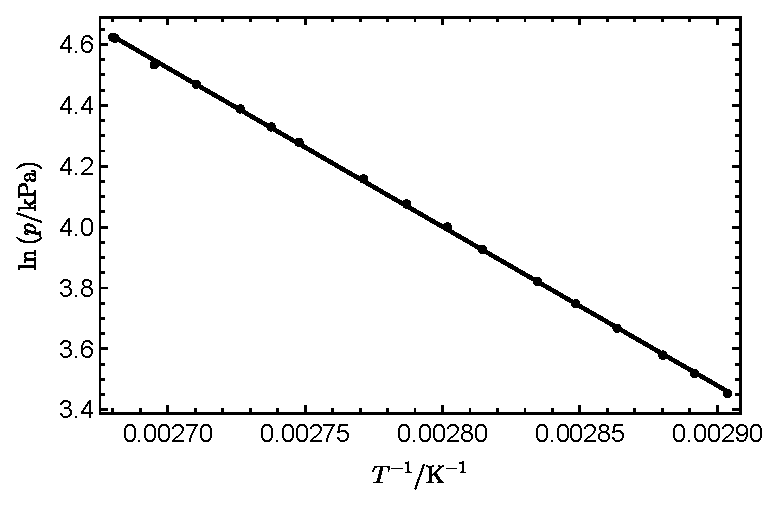
\includegraphics[width=0.45\textwidth]{figures/Clausiusfit.eps}
\caption{Data of the saturated vapor pressure of water fitted by $\ln{p}$ - $\frac{1}{T}$ curve}
\label{Clausius}
\end{figure}
\begin{figure}
\centering
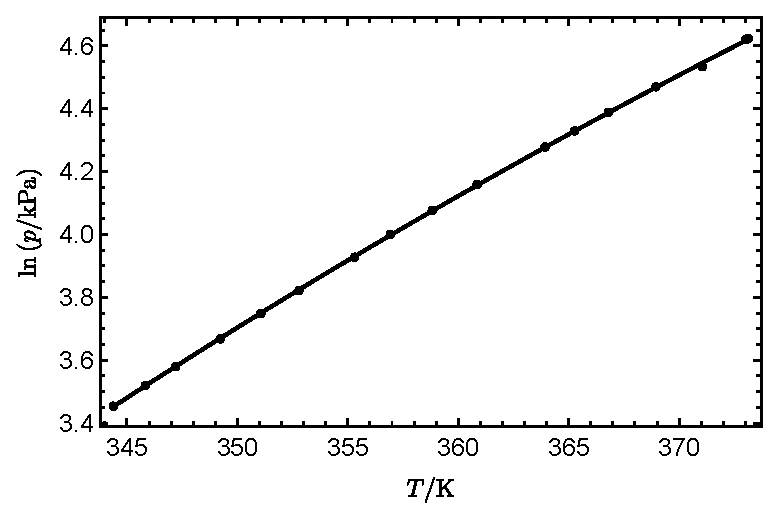
\includegraphics[width=0.45\textwidth]{figures/Antoinefit.eps}
\caption{Data of the saturated vapor pressure of water fitted using Antoine method}
\label{Antoine}
\end{figure}


The data recorded is shown in Table.\ref{waterdata}. The data is fitted using Clausius method and Antoine method perspectively, as shown in Fig.\ref{Clausius}. The line fitted is
\begin{equation}
\ln{(p/\mathrm{kPa})} = -5217 \times \frac{1}{T/\mathrm{K}} + 18.61
\end{equation}
with $R^2 = 0.999788$. Thus $\Delta_\text{vap} H_m^\ominus$ can be deduced, w.r.t. the fact that $\Delta_\text{vap}$ is assumed to be irrelevant with temperature,
\begin{equation}
\Delta_\text{vap} H_m^\ominus = 5278 \, \mathrm{K} \times R = \unit{43.37}{kJ/mol}
\end{equation}
 which is close to that given in the reference (44.00 kJ/mol\cite{franck1990jd}), verifying the deductions as well as assumptions given for the Clausius method. Deviation may arise from measurement error both during measuring temperature and pressure. Slight difference of temperature over the water during heating might also contribute to it by invalidating the invariability of $\Delta_\text{vap}H_m$, while deviation from equilibrium of pressure can also affect the result. It may also be considered that the water vapor may not completely follow the behaviors of an ideal gas, which makes the Clausius method does not give the explicit result. Further, the heat capacity of water changes at different temperature, which deviates $\Delta_\text{vap}$ from that in standard state.
\begin{equation}
\Delta_\text{vap}H_m^\ominus = 5278 \mathrm{K} \times R = \unit{43.88}{kJ/mol}
\end{equation}
Machine learning integrated in \emph{Mathematica} returns the result in Antoine method, namely
\begin{equation}
\ln{(p/\mathrm{kPa})} = A -\frac{B}{T-C}, \quad
\begin{cases}  
A=13.62,\\B=2250,\\C = 123.1
\end{cases}
\end{equation}
Thus
\begin{equation}
\Delta_\text{vap} H_m ^\ominus = \unit{54.24}{kJ/mol}, \Delta_\text{vap} S_m ^\ominus = \unit{181.9}{J/(mol \cdot K)}
\end{equation}
both of which does not match the data from reference. This might be due to the deficiency of accuracy describing the deviation in Antoine method, which simply treat the deviation as geometric series of $1/T$. It might also be due to inaccuracy in machine learning, whose complicated deduction of parameters may easily result in phenomena called `overfitting'. However, simple penalty function by introducing the norm of the parameters did not completely solve this problem, indicating a serious issue in this method.


\subsection{Measurement of decomposition equilibrium constant of ammonium carbamate}
The data recorded is shown in Table.\ref{acdata}. The line fitted is 
\begin{equation}
\ln{(p/\mathrm{kPa})} = -6491 \times \frac{1}{T/\mathrm{K}} + 24.23
\end{equation}
with $R^2 = 0.999795$. Considering that
\begin{equation}
p_\text{\ce{CO2}} = \frac{1}{3} p_\text{total}, p_\text{\ce{NH3}} = \frac{2}{3} p_\text{total}
\end{equation}
it is easily deduced that
\begin{equation}
\ln{K^\ominus} = 3 \ln{p} + \mathrm{constant}
\end{equation}
thus
\begin{equation}
\Delta_r H_m^\ominus = \unit{161.9}{kJ/mol}
\end{equation}
Unfortunately, data from references cannot be searched. Great linearity is achieved, verifying the model provided for this reaction. Sources of deviations resembles the experiment in the measurement of saturated vapor pressure of water, including the non-ideal-gas behavior, failure to reach the chemical equilibrium, as well as measurement error.

\begin{table}
\centering
\caption{Data collected in the measurment of decomposition equilibrium constant of ammonium carbamate}
\begin{tabular}{cc}\hline
$T$/K & $p$/kPa \\\hline
 298.15 & 11.63 \\
 303.15 & 16.91 \\
 308.15 & 23.89 \\
 313.15 & 33.46 \\
 318.16 & 45.74 \\\hline
\end{tabular}
\label{acdata}
\end{table}

\section{Conclusions}
From the equations and the experiment results we observe an intimate relation between equilibrium and temperature, which is due to the sophisticated connection between energy and entropy. Assumption of ideal-gas behavior in the gas phase of the products as well as the indifference of deviation of $\Delta_r H_m$ towards temperature leads to linearity of $\ln{p}$ or $\ln{K}$ towards $\frac{1}{T}$, which is successfully verified by experiments. 

\bibliography{References}

\end{document}
